%%%%% Jornadas Sarteco 2026 — CASTM: ZKP Kernels on CGRA %%%%%%

\documentclass[twocolumn,twoside]{Jornadas}
\usepackage[utf8]{inputenc}
\usepackage[spanish,es-noshorthands]{babel}
\usepackage{listings}
\usepackage{algorithm}
\usepackage{algorithmicx}
\usepackage{algcompatible}
\usepackage{adjustbox}
\usepackage{graphicx}
\usepackage{color}
\usepackage{xcolor}
\usepackage{caption}
\captionsetup{font=footnotesize}
\usepackage[caption=false,font=footnotesize]{subfig}
\usepackage{placeins}
\usepackage{hyperref}
\hypersetup{hidelinks}
\usepackage{url}
\usepackage{amsmath,amssymb,mathtools}
\usepackage{booktabs}
\usepackage{array}
\usepackage{multirow}
\usepackage{float}
\usepackage{tikz}
\usepackage{makecell}
\usetikzlibrary{shapes,arrows,positioning,calc,fit,backgrounds,matrix,arrows.meta,shapes.geometric,patterns,decorations.pathreplacing,babel,chains}

% -*- Ajustes LaTeX en relación a las figuras -*-
\setcounter{topnumber}{10}
\setcounter{bottomnumber}{10}
\setcounter{totalnumber}{10}
\renewcommand{\topfraction}{1}
\renewcommand{\bottomfraction}{1}
\renewcommand{\textfraction}{0}
\renewcommand{\floatpagefraction}{1}

% ── Color palette ──
\definecolor{cgrablue}{HTML}{2563EB}
\definecolor{cgragreen}{HTML}{16A34A}
\definecolor{cgrared}{HTML}{DC2626}
\definecolor{cgraorange}{HTML}{EA580C}
\definecolor{cgrapurple}{HTML}{9333EA}
\definecolor{cgragray}{HTML}{6B7280}
\definecolor{cgralabel}{HTML}{7C2D12}
\definecolor{cgraaddr}{HTML}{9A3412}
\definecolor{cgralight}{HTML}{EFF6FF}
\definecolor{codebg}{HTML}{F8FAFC}

\definecolor{gray97}{gray}{.97}
\definecolor{gray75}{gray}{.75}
\definecolor{gray45}{gray}{.45}

% ── Listings: OpenEdge DSL ──
\lstdefinelanguage{edsl}{
  alsoletter={_},
  morekeywords=[1]{target,build,optimize,scheduler,kernel,function,cycle,bundle,at,all,for,in,range,let,if,else,while,goto,io,load,store},
  morekeywords=[2]{EXIT,NOP,BSFA,BZFA,LWI,SWI,SADD,SSUB,SMUL,JUMP,ROUT,SELF,RCL,RCR,RCT,RCB,ZERO,R0,R1,R2,R3},
  morekeywords=[3]{std,extract_bytes,extract_bytes_col,extract_bytes_row,carry_chain,broadcast,normalize,reduce,route,stash},
  morekeywords=[4]{subrA,subrB,subrC,ret1,ret3},
  sensitive=true,
  morecomment=[l]{//},
  morecomment=[s]{/*}{*/},
  morestring=[b]",
  moredelim=*[s][\bfseries\itshape\color{cgraaddr}]{@}{:},
  literate={std::}{{\textcolor{cgrapurple}{std::}}}5,
}

\lstset{
  language=edsl,
  inputencoding=utf8,
  extendedchars=true,
  basicstyle=\ttfamily\scriptsize,
  keywordstyle=[1]\bfseries\color{cgrablue},
  keywordstyle=[2]\color{cgrared},
  keywordstyle=[3]\color{cgrapurple},
  keywordstyle=[4]\bfseries\color{cgralabel},
  commentstyle=\itshape\color{cgragreen!70!black},
  stringstyle=\color{cgraorange},
  numbers=left,
  numberstyle=\tiny\color{cgragray},
  numbersep=5pt,
  frame=single,
  rulecolor=\color{cgragray!40},
  backgroundcolor=\color{codebg},
  breaklines=true,
  captionpos=b,
  tabsize=4,
  columns=flexible,
  linewidth=.98\columnwidth,
  xleftmargin=3mm,
  aboveskip=8pt,
  belowskip=4pt,
  escapeinside={(*@}{@*)},
  literate={á}{{\'a}}1 {é}{{\'e}}1 {í}{{\'i}}1 {ó}{{\'o}}1 {ú}{{\'u}}1 {ñ}{{\~n}}1,
}

% ── Listings: CSV raw format ──
\lstdefinelanguage{csvraw}{
  basicstyle=\ttfamily\scriptsize\color{cgragray!80!black},
  frame=single,
  rulecolor=\color{cgragray!40},
  backgroundcolor=\color{cgrared!3},
  numbers=left,
  numberstyle=\tiny\color{cgragray},
  numbersep=5pt,
  breaklines=true,
  captionpos=b,
  xleftmargin=3mm,
}

\def\BibTeX{{\rm B\kern-.05em{\sc i\kern-.025em b}\kern-.08em
    T\kern-.1667em\lower.7ex\hbox{E}\kern-.125emX}}

\newcommand{\babybear}{p = 2^{31} - 2^{27} + 1}
\newcommand{\NCC}{N_{\mathrm{CC}}}
\newcommand{\Mod}{\operatorname{mod}}
\newcommand{\castm}{CASTM}
\newcommand{\placeholder}[1]{\colorbox{yellow!30}{\textit{#1}}}
\newcommand{\statmin}{\operatorname{min}}
\newcommand{\cc}[1]{#1~CC}
\newcommand{\pct}[1]{#1\%}
\newcommand{\timex}[1]{#1$\times$}
\newcommand{\ujperm}[1]{#1~$\mu$J/perm}
\newcommand{\nj}[1]{#1\,nJ}
\newcommand{\lines}[1]{#1~lines}
\newcommand{\kpermperj}[1]{#1~kperm/J}
\newcommand{\mw}[1]{#1\,mW}

% Centralized paper metrics layer.
% Manual paper metrics without a stable machine-readable upstream source.
% Keep this file small: only values that cannot yet be derived from the
% canonical research artifacts should live here.
% Maintenance guide: METRICS.md
% Do not duplicate values already exported into generated/paper_metrics_auto.tex.

% Intro / walkthrough
\newcommand{\MetricSboxKernelManualAuthoringTime}{two weeks}
\newcommand{\MetricSboxKernelComputeCC}{205}
\newcommand{\MetricSboxKernelBarrettSharePct}{76}
\newcommand{\MetricSboxKernelSubrABundles}{39}
\newcommand{\MetricSboxKernelSubrACalls}{4}
\newcommand{\MetricSboxKernelSharedBundlesSaved}{156}
\newcommand{\MetricSboxKernelApproxPreReuseBundles}{700}
\newcommand{\MetricSboxKernelResidentBundles}{73}

% CRF sizing study — depths and hardware cost
\newcommand{\MetricCrfDefaultDepth}{32}
\newcommand{\MetricCrfDepthSixtyFour}{64}
\newcommand{\MetricCrfDepthOneTwentyEight}{128}
\newcommand{\MetricCrfDepthTwoFiftySix}{256}
\newcommand{\MetricCrfDepthFullFit}{512}

\newcommand{\MetricCrfSixtyFourExtraFlipFlops}{16{,}384}
\newcommand{\MetricCrfOneTwentyEightExtraFlipFlops}{49{,}152}
\newcommand{\MetricCrfTwoFiftySixExtraFlipFlops}{114{,}688}
\newcommand{\MetricCrfFullFitExtraFlipFlops}{245{,}760}

\newcommand{\MetricCrfSixtyFourAreaPct}{0.3}
\newcommand{\MetricCrfOneTwentyEightAreaPct}{0.9}
\newcommand{\MetricCrfTwoFiftySixAreaPct}{2.1}
\newcommand{\MetricCrfFullFitAreaPct}{4.5}

% CRF overhead — Manual kernel (406 NB, 678 CC exec, flat/partitionable)
% Model: OH = CONF + FSM + set_kernel + CMEM_reload (RTL-traced)
\newcommand{\MetricCrfManualDefaultK}{13}
\newcommand{\MetricCrfManualDefaultOH}{6{,}770}
\newcommand{\MetricCrfManualDefaultTotal}{7{,}448}
\newcommand{\MetricCrfManualDefaultOHPct}{91}
\newcommand{\MetricCrfManualSixtyFourK}{7}
\newcommand{\MetricCrfManualSixtyFourOH}{6{,}612}
\newcommand{\MetricCrfManualSixtyFourTotal}{7{,}290}
\newcommand{\MetricCrfManualSixtyFourOHPct}{91}
\newcommand{\MetricCrfManualOneTwentyEightK}{4}
\newcommand{\MetricCrfManualOneTwentyEightOH}{6{,}485}
\newcommand{\MetricCrfManualOneTwentyEightTotal}{7{,}163}
\newcommand{\MetricCrfManualOneTwentyEightOHPct}{91}
\newcommand{\MetricCrfManualTwoFiftySixK}{2}
\newcommand{\MetricCrfManualTwoFiftySixOH}{4{,}267}
\newcommand{\MetricCrfManualTwoFiftySixTotal}{4{,}945}
\newcommand{\MetricCrfManualTwoFiftySixOHPct}{86}
\newcommand{\MetricCrfManualFullFitK}{1}
\newcommand{\MetricCrfManualFullFitOH}{0}
\newcommand{\MetricCrfManualFullFitTotal}{678}
\newcommand{\MetricCrfManualFullFitOHPct}{0}

% CRF overhead — CASTM kernel (73 NB, 539 CC exec, jump-reuse/non-partitionable)
\newcommand{\MetricCrfCastmDefaultK}{3}
\newcommand{\MetricCrfCastmDefaultOH}{1{,}107}
\newcommand{\MetricCrfCastmDefaultTotal}{1{,}646}
\newcommand{\MetricCrfCastmDefaultOHPct}{67}
\newcommand{\MetricCrfCastmSixtyFourK}{2}
\newcommand{\MetricCrfCastmSixtyFourOH}{1{,}054}
\newcommand{\MetricCrfCastmSixtyFourTotal}{1{,}593}
\newcommand{\MetricCrfCastmSixtyFourOHPct}{66}
\newcommand{\MetricCrfCastmOneTwentyEightK}{1}
\newcommand{\MetricCrfCastmOneTwentyEightOH}{0}
\newcommand{\MetricCrfCastmOneTwentyEightTotal}{539}
\newcommand{\MetricCrfCastmOneTwentyEightOHPct}{0}

% Auto-generated by submodules/poseidon2/scripts/analysis/export_europar2026_metrics.py
% Do not edit by hand; regenerate from the canonical research artifacts.
% Maintenance guide: papers/Cristian-EuroPar2026/METRICS.md

\newcommand{\MetricHalsteadCastmRatio}{6.4}
\newcommand{\MetricHalsteadCompigraRatio}{2.4}
\newcommand{\MetricHalsteadCompressionVsManual}{10.10}
\newcommand{\MetricHalsteadCppRefRatio}{1.0}
\newcommand{\MetricHalsteadManualRatio}{64.5}
\newcommand{\MetricLocCastm}{340}
\newcommand{\MetricLocCompigra}{47}
\newcommand{\MetricLocCompressionVsManual}{6.0}
\newcommand{\MetricLocCppRef}{25}
\newcommand{\MetricLocManual}{2{,}030}
\newcommand{\MetricRtlCgraClockMHz}{100}
\newcommand{\MetricRtlCgraOnlyCC}{56{,}416}
\newcommand{\MetricRtlCgraOnlyCgraEnergyUJ}{2.993}
\newcommand{\MetricRtlCgraOnlyCpuEnergyUJ}{0.012}
\newcommand{\MetricRtlCgraOnlyEEKpermPerJ}{332.8}
\newcommand{\MetricRtlCgraOnlyEnergyReductionPct}{34.5}
\newcommand{\MetricRtlCgraOnlyOneToMCC}{68{,}643}
\newcommand{\MetricRtlCgraOnlyOneToMSpeedupReal}{1.08}
\newcommand{\MetricRtlCgraOnlySpeedupReal}{1.30}
\newcommand{\MetricRtlCgraOnlyTimeUs}{564.2}
\newcommand{\MetricRtlCgraOnlyTotalEnergyUJ}{3.005}
\newcommand{\MetricRtlCpuClockMHz}{250}
\newcommand{\MetricRtlCpuOnlyCC}{183{,}591}
\newcommand{\MetricRtlCpuOnlyCpuEnergyUJ}{4.588}
\newcommand{\MetricRtlCpuOnlyEEKpermPerJ}{217.9}
\newcommand{\MetricRtlCpuOnlySpeedupReal}{1.00}
\newcommand{\MetricRtlCpuOnlyTimeUs}{734.4}
\newcommand{\MetricRtlCpuOnlyTotalEnergyUJ}{4.588}
\newcommand{\MetricRtlCpuPowerModelMW}{2.5}
\newcommand{\MetricRtlHybridCC}{67{,}717}
\newcommand{\MetricRtlHybridCgraEnergyUJ}{1.390}
\newcommand{\MetricRtlHybridCpuEnergyUJ}{0.021}
\newcommand{\MetricRtlHybridEEKpermPerJ}{708.6}
\newcommand{\MetricRtlHybridEnergyReductionPct}{69.2}
\newcommand{\MetricRtlHybridSpeedupReal}{1.08}
\newcommand{\MetricRtlHybridTimeUs}{677.2}
\newcommand{\MetricRtlHybridTotalEnergyUJ}{1.411}
\newcommand{\MetricSboxCastmCC}{539}
\newcommand{\MetricSboxCastmCsvBundleCount}{73}
\newcommand{\MetricSboxCastmCsvLastBundleIndex}{72}
\newcommand{\MetricSboxCastmCsvLines}{365}
\newcommand{\MetricSboxCastmCycleReductionPct}{20.5}
\newcommand{\MetricSboxCastmDispatches}{1}
\newcommand{\MetricSboxCastmEnergyNJ}{4.65}
\newcommand{\MetricSboxCastmEnergyUJ}{0.005}
\newcommand{\MetricSboxCastmIdleArithmeticPct}{60.0}
\newcommand{\MetricSboxCastmIdlePct}{41.7}
\newcommand{\MetricSboxCastmKernelNB}{73}
\newcommand{\MetricSboxCastmNB}{73}
\newcommand{\MetricSboxCastmPowerMW}{0.86}
\newcommand{\MetricSboxCastmSmulPct}{4.1}
\newcommand{\MetricSboxCastmSpeedupVsManual}{1.26}
\newcommand{\MetricSboxCompigraCC}{3{,}544}
\newcommand{\MetricSboxCompigraCsvBundleCount}{2{,}564}
\newcommand{\MetricSboxCompigraCsvLastBundleIndex}{2{,}563}
\newcommand{\MetricSboxCompigraCsvLines}{12{,}820}
\newcommand{\MetricSboxCompigraDispatches}{244}
\newcommand{\MetricSboxCompigraEnergyNJ}{26.69}
\newcommand{\MetricSboxCompigraEnergyUJ}{0.027}
\newcommand{\MetricSboxCompigraIdleArithmeticPct}{90.2}
\newcommand{\MetricSboxCompigraIdlePct}{89.9}
\newcommand{\MetricSboxCompigraKernelNB}{21}
\newcommand{\MetricSboxCompigraNB}{2{,}564}
\newcommand{\MetricSboxCompigraPowerMW}{0.75}
\newcommand{\MetricSboxCompigraSlowdownVsCastm}{6.58}
\newcommand{\MetricSboxCompigraSmulPct}{0.0}
\newcommand{\MetricSboxManualCC}{678}
\newcommand{\MetricSboxManualCsvBundleCount}{406}
\newcommand{\MetricSboxManualCsvLastBundleIndex}{405}
\newcommand{\MetricSboxManualDispatches}{1}
\newcommand{\MetricSboxManualEnergyNJ}{6.26}
\newcommand{\MetricSboxManualEnergyUJ}{0.006}
\newcommand{\MetricSboxManualIdleArithmeticPct}{74.6}
\newcommand{\MetricSboxManualIdlePct}{64.3}
\newcommand{\MetricSboxManualKernelNB}{406}
\newcommand{\MetricSboxManualNB}{406}
\newcommand{\MetricSboxManualPowerMW}{0.92}
\newcommand{\MetricSboxManualSmulPct}{2.5}
\newcommand{\MetricValidationEdslMismatches}{0}
\newcommand{\MetricValidationEdslVectors}{104}
\newcommand{\MetricValidationSboxMismatches}{0}
\newcommand{\MetricValidationSboxVectors}{25}

% Auto-generated by export_cgra_poseidon2_eval_metrics.py
\newcommand{\MetricMerkleLeaves}{16}
\newcommand{\MetricMerkleHashes}{15}
\newcommand{\MetricMerkleCpuClockMHz}{100}
\newcommand{\MetricMerkleCgraClockMHz}{100}
\newcommand{\MetricMerkleWallTimerMHz}{100}
\newcommand{\MetricMerkleProjCpuClockMHz}{250}
\newcommand{\MetricMerkleProjCgraClockMHz}{100}
\newcommand{\MetricMerkleCpuPowerModelMW}{2.5}
\newcommand{\MetricMerkleCoexecSchedPolicy}{legacy-50-50}
\newcommand{\MetricMerkleCoexecSchedCgraSharePct}{50}
\newcommand{\MetricMerkleCoexecSchedCpuSharePct}{50}
\newcommand{\MetricMerkleCoexecSchedProjCpuEqOneHundredCC}{73{,}661}
\newcommand{\MetricMerkleCoexecSchedReferenceCgraCC}{55{,}686}
\newcommand{\MetricMerkleCpuOnlyCC}{2{,}750{,}358}
\newcommand{\MetricMerkleCpuOnlyCpuCC}{2{,}750{,}427}
\newcommand{\MetricMerkleCpuOnlyCgraCC}{0}
\newcommand{\MetricMerkleCpuOnlyCgraProductiveCC}{0}
\newcommand{\MetricMerkleCpuOnlyCgraStallCC}{0}
\newcommand{\MetricMerkleCpuOnlyTotalCC}{2{,}750{,}358}
\newcommand{\MetricMerkleCpuOnlyTimeUs}{27{,}503.6}
\newcommand{\MetricMerkleCpuOnlyTimeMs}{27.504}
\newcommand{\MetricMerkleCpuOnlySpeedup}{1.00}
\newcommand{\MetricMerkleCpuOnlyProjectedSpeedup}{1.00}
\newcommand{\MetricMerkleCpuOnlyHashesPerSec}{545}
\newcommand{\MetricMerkleCpuOnlyProjectedCpuTimeUs}{11{,}001.7}
\newcommand{\MetricMerkleCpuOnlyProjectedCpuTimeMs}{11.002}
\newcommand{\MetricMerkleCpuOnlyProjectedCgraTimeUs}{0.0}
\newcommand{\MetricMerkleCpuOnlyProjectedCgraTimeMs}{0.000}
\newcommand{\MetricMerkleCpuOnlyProjectedTimeUs}{11{,}001.4}
\newcommand{\MetricMerkleCpuOnlyProjectedTimeMs}{11.001}
\newcommand{\MetricMerkleCpuOnlyProjectedHashesPerSec}{1{,}363}
\newcommand{\MetricMerkleCpuOnlyProjectedCpuTimePerHashUs}{733.4}
\newcommand{\MetricMerkleCpuOnlyProjectedCgraTimePerHashUs}{0.0}
\newcommand{\MetricMerkleCpuOnlyProjectedTimePerHashUs}{733.4}
\newcommand{\MetricMerkleCpuOnlyCpuEnergyPerHashUJ}{4.584}
\newcommand{\MetricMerkleCpuOnlyCgraEnergyPerHashUJ}{0.000}
\newcommand{\MetricMerkleCpuOnlyTotalEnergyPerHashUJ}{4.584}
\newcommand{\MetricMerkleCpuOnlyCpuEnergyUJ}{68.761}
\newcommand{\MetricMerkleCpuOnlyCgraEnergyUJ}{0.000}
\newcommand{\MetricMerkleCpuOnlyTotalEnergyUJ}{68.761}
\newcommand{\MetricMerkleCpuOnlyEnergySavingsPct}{0.0}
\newcommand{\MetricMerkleCpuOnlyKernels}{0}
\newcommand{\MetricMerkleCpuOnlyWfiCC}{0}
\newcommand{\MetricMerkleCpuOnlyDsideWaitCC}{49{,}650}
\newcommand{\MetricMerkleCpuOnlyMemLoad}{36{,}575}
\newcommand{\MetricMerkleCpuOnlyMemStore}{13{,}069}
\newcommand{\MetricMerkleCoexecCC}{1{,}343{,}712}
\newcommand{\MetricMerkleCoexecCpuCC}{1{,}343{,}783}
\newcommand{\MetricMerkleCoexecCgraCC}{436{,}164}
\newcommand{\MetricMerkleCoexecCgraProductiveCC}{436{,}164}
\newcommand{\MetricMerkleCoexecCgraStallCC}{0}
\newcommand{\MetricMerkleCoexecTotalCC}{1{,}343{,}712}
\newcommand{\MetricMerkleCoexecTimeUs}{13{,}437.1}
\newcommand{\MetricMerkleCoexecTimeMs}{13.437}
\newcommand{\MetricMerkleCoexecSpeedup}{2.05}
\newcommand{\MetricMerkleCoexecProjectedSpeedup}{2.05}
\newcommand{\MetricMerkleCoexecHashesPerSec}{1{,}116}
\newcommand{\MetricMerkleCoexecProjectedCpuTimeUs}{5{,}375.1}
\newcommand{\MetricMerkleCoexecProjectedCpuTimeMs}{5.375}
\newcommand{\MetricMerkleCoexecProjectedCgraTimeUs}{4{,}361.6}
\newcommand{\MetricMerkleCoexecProjectedCgraTimeMs}{4.362}
\newcommand{\MetricMerkleCoexecProjectedTimeUs}{5{,}374.8}
\newcommand{\MetricMerkleCoexecProjectedTimeMs}{5.375}
\newcommand{\MetricMerkleCoexecProjectedHashesPerSec}{2{,}791}
\newcommand{\MetricMerkleCoexecProjectedCpuTimePerHashUs}{358.3}
\newcommand{\MetricMerkleCoexecProjectedCgraTimePerHashUs}{290.8}
\newcommand{\MetricMerkleCoexecProjectedTimePerHashUs}{358.3}
\newcommand{\MetricMerkleCoexecCpuEnergyPerHashUJ}{2.240}
\newcommand{\MetricMerkleCoexecCgraEnergyPerHashUJ}{1.596}
\newcommand{\MetricMerkleCoexecTotalEnergyPerHashUJ}{3.836}
\newcommand{\MetricMerkleCoexecCpuEnergyUJ}{33.595}
\newcommand{\MetricMerkleCoexecCgraEnergyUJ}{23.940}
\newcommand{\MetricMerkleCoexecTotalEnergyUJ}{57.535}
\newcommand{\MetricMerkleCoexecEnergySavingsPct}{16.3}
\newcommand{\MetricMerkleCoexecKernels}{8}
\newcommand{\MetricMerkleCoexecWfiCC}{0}
\newcommand{\MetricMerkleCoexecDsideWaitCC}{33{,}626}
\newcommand{\MetricMerkleCoexecMemLoad}{26{,}857}
\newcommand{\MetricMerkleCoexecMemStore}{6{,}683}
\newcommand{\MetricMerkleOffloadCC}{842{,}916}
\newcommand{\MetricMerkleOffloadCpuCC}{27{,}902}
\newcommand{\MetricMerkleOffloadCgraCC}{815{,}310}
\newcommand{\MetricMerkleOffloadCgraProductiveCC}{815{,}310}
\newcommand{\MetricMerkleOffloadCgraStallCC}{0}
\newcommand{\MetricMerkleOffloadTotalCC}{842{,}916}
\newcommand{\MetricMerkleOffloadTimeUs}{8{,}429.2}
\newcommand{\MetricMerkleOffloadTimeMs}{8.429}
\newcommand{\MetricMerkleOffloadSpeedup}{3.26}
\newcommand{\MetricMerkleOffloadProjectedSpeedup}{1.33}
\newcommand{\MetricMerkleOffloadHashesPerSec}{1{,}779}
\newcommand{\MetricMerkleOffloadProjectedCpuTimeUs}{111.6}
\newcommand{\MetricMerkleOffloadProjectedCpuTimeMs}{0.112}
\newcommand{\MetricMerkleOffloadProjectedCgraTimeUs}{8{,}153.1}
\newcommand{\MetricMerkleOffloadProjectedCgraTimeMs}{8.153}
\newcommand{\MetricMerkleOffloadProjectedTimeUs}{8{,}261.7}
\newcommand{\MetricMerkleOffloadProjectedTimeMs}{8.262}
\newcommand{\MetricMerkleOffloadProjectedHashesPerSec}{1{,}816}
\newcommand{\MetricMerkleOffloadProjectedCpuTimePerHashUs}{7.4}
\newcommand{\MetricMerkleOffloadProjectedCgraTimePerHashUs}{543.5}
\newcommand{\MetricMerkleOffloadProjectedTimePerHashUs}{550.8}
\newcommand{\MetricMerkleOffloadCpuEnergyPerHashUJ}{0.047}
\newcommand{\MetricMerkleOffloadCgraEnergyPerHashUJ}{2.993}
\newcommand{\MetricMerkleOffloadTotalEnergyPerHashUJ}{3.039}
\newcommand{\MetricMerkleOffloadCpuEnergyUJ}{0.698}
\newcommand{\MetricMerkleOffloadCgraEnergyUJ}{44.888}
\newcommand{\MetricMerkleOffloadTotalEnergyUJ}{45.585}
\newcommand{\MetricMerkleOffloadEnergySavingsPct}{33.7}
\newcommand{\MetricMerkleOffloadKernels}{15}
\newcommand{\MetricMerkleOffloadWfiCC}{90}
\newcommand{\MetricMerkleOffloadDsideWaitCC}{8{,}454}
\newcommand{\MetricMerkleOffloadMemLoad}{3{,}856}
\newcommand{\MetricMerkleOffloadMemStore}{2{,}837}


%Directorios en los que se buscan las figuras
\graphicspath{{.}{./Figuras/}{./figures/}}
%%%%%%%%%%%%%%%%%%%%%%%%%%%%%%%%%%%%%%%%%%%%

\begin{document}

\title{Accelerating Zero-Knowledge Proof Kernels on CGRA Architectures}

\author{%
     Cristian Campos Ferrer, Ángeles G.\ Navarro y Sonia González-Navarro%
     \thanks{Dpto.\ de Arquitectura de Computadores, Universidad de Málaga,
     e-mail: {\tt \{cricamfe,angeles,sonia\}@ac.uma.es}}
}

\maketitle
\markboth{}{}
\pagestyle{empty}
\thispagestyle{empty}

%% ANTIGUO ABSTRACT
% \begin{abstract}
% Wearable biomedical devices increasingly require on-device privacy guarantees through Zero-Knowledge Proofs~(ZKPs), yet the underlying cryptographic kernels, based on modular exponentiation over prime fields, far exceed what low-power microcontrollers can deliver. Coarse-Grained Reconfigurable Arrays~(CGRAs) offer near-ASIC efficiency with the reprogrammability needed to track evolving ZKP standards, but programming them requires manual, cycle-by-cycle scheduling across a spatial processing-element mesh.
% %
% We present \castm{}, a \textit{CGRA API} \& \textit{Spatial Temporal Mapper} for the OpenEdgeCGRA architecture. \castm{} preserves explicit spatial-temporal control while raising the abstraction level through structured abstractions and architecture-aware operators that encapsulate recurring modular-arithmetic idioms. For the S-box layer, a key component of the popular ZKP-friendly hash function Poseidon2, \castm{} achieves \timex{\MetricSboxCastmSpeedupVsManual} speedup w.r.t.\ the hand-optimized version while reducing source code by approximately \timex{\MetricLocCompressionVsManual}.
% We also identify that for long ZKP kernels multi-batch configuration reload is the dominant bottleneck, and show that increasing the Configuration Register File from 32 to 512 entries (+\pct{\MetricCrfFullFitAreaPct} FPGA area) allow us to deploy the full Poseidon2 kernel on the CGRA achieving \timex{\MetricMerkleOffloadProjectedSpeedup} speedup and \MetricMerkleOffloadEnergySavingsPct\% of energy savings over a ultra-low power RISC-V CPU core.
% \end{abstract}

%% POSIBLE MUEVO ABSTRACT
\begin{abstract}
Wearable biomedical devices increasingly require on-device privacy guarantees through Zero-Knowledge Proofs~(ZKPs), yet the underlying cryptographic kernels, based on modular exponentiation over prime fields, far exceed what low-power microcontrollers can deliver. Coarse-Grained Reconfigurable Arrays~(CGRAs) offer near-ASIC efficiency with the reprogrammability needed to track evolving ZKP standards, but programming them requires cycle-by-cycle scheduling across a spatial processing-element mesh.
%
We present an efficient spatial-temporal mapping of the S-box layer ($x^7 \Mod p$, BabyBear) of the ZKP-friendly hash function Poseidon2 onto the OpenEdgeCGRA architecture, a $4{\times}4$ toroidal PE mesh. The mapping leverages the mesh topology to perform Barrett modular reduction entirely through inter-PE communication, reducing the memory-access stalls that limit naive approaches. Through subroutine reuse of the Barrett reduction phase, fall-through chaining, and instruction merging across PEs, the S-box kernel achieves \timex{\MetricSboxCastmSpeedupVsManual} speedup w.r.t.\ a hand-optimized flat schedule and \timex{\MetricSboxCompigraSlowdownVsCastm} over an automatic compiler.
We also identify that for long ZKP kernels multi-batch configuration reload is the dominant bottleneck, and show that increasing the Configuration Register File from 32 to 512 entries (+\pct{\MetricCrfFullFitAreaPct} FPGA area) enables deploying the full Poseidon2 kernel on the CGRA, achieving \timex{\MetricMerkleOffloadProjectedSpeedup} speedup and \MetricMerkleOffloadEnergySavingsPct\% energy savings over an ultra-low power RISC-V CPU core.
\end{abstract}

\begin{keywords}
OpenEdgeCGRA, Zero-Knowledge Proofs, Poseidon2.
\end{keywords}

%!TEX root = main.tex
\section{Introduction}
\label{sec:introduction}

\PARstart{W}{earable} biomedical devices---continuous glucose monitors, cardiac rhythm analyzers, inertial fall predictors---generate vast amounts of physiological data transmitted wirelessly to cloud platforms~\cite{wearable-health}. Regulatory frameworks (HIPAA, GDPR) impose strict requirements on data provenance, yet current device architectures lack mechanisms for the device itself to \emph{prove} that a measurement is authentic without revealing raw signals. Zero-Knowledge Proofs (ZKPs)~\cite{groth16,plonk} resolve this tension: a prover (the sensor) convinces a verifier (a server) that a statement holds---e.g., that a glucose trajectory was computed correctly---without disclosing the underlying data. Elliptic Curve Cryptography (ECC)~\cite{ecc-iot} underpins the most compact constructions, keeping proof sizes small for bandwidth-constrained links.

Deploying ZKP on hardware demands \emph{reconfigurability}. Different proof systems (Groth16~\cite{groth16}, PLONK~\cite{plonk}, STARKs~\cite{stark-anatomy}) use different prime fields (31-bit BabyBear, 64-bit Goldilocks, 256-bit BN254), S-box exponents ($d\!\in\!\{3,5,7\}$), and elliptic curves. Plonky3~\cite{babybear} introduced BabyBear only in 2024, replacing the Goldilocks field of Plonky2. An ASIC designed for one configuration becomes obsolete when the next proof system changes parameters. Coarse-Grained Reconfigurable Arrays (CGRAs) occupy the right design point: unlike FPGAs, they reconfigure at the instruction level with microsecond latency; unlike ASICs, they remain fully reprogrammable~\cite{cgra-survey}. In our research, we target the X-HEEP framework~\cite{xheep}, an extensible
RISC-V based SoC designed for ultra low power edge computing, capable of interfacing with custom peripherals like accelerators. In particular, applications of the X-HEEP framework, such as  HEEPocrates and HEEPsilon feature a CGRA integrated via the Extendible Accelerator Interface (XAIF): the OpenEdgeCGRA~\cite{openedge-cgra},
a $4 \times 4$ PE mesh with a 32-bit datapath,
which we consider in this paper.

The computational bottleneck in ZKP is the hash function. We focus our research on the Poseidon2 framework~\cite{poseidon2}, which implement a hash that minimizes finite-field multiplications per permutation making it highly suitable for our data privacy use case (a biomedical wereable). In any case, its S-box layer---$x^d \Mod p$---accounts for over 90\% of computation on a CGRA with 32-bit datapath. For 31-bit BabyBear ($\babybear$, $d\!=\!7$), each S-box requires two modular squarings and two modular multiplications, each involving Barrett reduction~\cite{barrett1986} with 62-bit intermediates decomposed across 32-bit PEs. Yet programming the CGRA is the real bottleneck: the developer must specify, for each of the $N\times M$~PEs and each clock cycle, the exact instruction, registers, and neighbor links. For the S-box layer this spans \lines{\MetricLocManual}, took \MetricSboxKernelManualAuthoringTime{} of expert effort, and a single misplaced operand produces silent errors detectable only through full simulation. Automatic compilers~\cite{compigra,wang2025mlir} avoid this burden but cannot express cross-PE carry chains, toroidal routing, or branchless conditional selects that are essential for modular arithmetic.

In this paper we present \castm{} (CGRA API \& Spatial Temporal Mapper),
which occupies the middle ground: the programmer retains explicit control over \emph{which PE} executes \emph{which instruction} at \emph{which cycle}, but through parametric functions, loops, labeled subroutines, and architecture-aware operators instead of raw CSV encodings. A four-stage deterministic pipeline
produces simulator-native CSV with structured error diagnostics. More precisely, we make the following contributions: \textbf{(C1)} We introduce \castm{}, the first API targeting spatial-temporal CGRA programming for cryptographic workloads (Section~\ref{sec:openedge}).
\textbf{(C2)} We map S-box layer ($x^7 \Mod p$, BabyBear) onto OpenEdgeCGRA and validate the resulting flow against independent C/C++ references (Section~\ref{subsec:sbox-openedge}). \textbf{(C3)} We show \castm{} reduces source code by approximately \timex{\MetricLocCompressionVsManual} vs.\ manual CSV while achieving \pct{\MetricSboxCastmCycleReductionPct} fewer clock cycles on the S-box kernel (Section~\ref{subsec:sbox-comparison}). \textbf{(C4)} We identify multi-batch configuration reload as the dominant bottleneck and evaluate increasing Configuration Register File --CRF-- capacity to enable full Poseidon2 deployment on CGRA (Section~\ref{subsec:creg-analysis}). \textbf{(C5)} We show that throughput and energy favor different deployments of Poseidon2 on the CPU and the CGRA (Section~\ref{subsec:rtl-poseidon2}).

%!TEX root = main.tex
\section{Background and Related Work}
\label{sec:background}

\subsection{OpenEdgeCGRA Architecture}
\label{subsec:cgra-basics}

Coarse Grained Reconfigurable Arrays (CGRAs) are primarily composed of an array of interconnected
PEs (or Reconfigurable Cells --RCs--) that can be configured dynamically to implement a variety of computational tasks. The PEs are connected through a fixed interconnect, executing in lockstep under a configuration bitstream loaded before kernel execution~\cite{cgra-survey}. Each PE contains a word-width ALU, a small register file, and neighbor connections. Unlike FPGAs (bit-level reconfiguration, high overhead), CGRAs reconfigure at the instruction level with microsecond latency.

OpenEdgeCGRA~\cite{openedge-cgra} provides: \textit{(i)} a $4\times4$ toroidal mesh of PEs (i.e 16 PEs),  where column~3 wraps to column~0 and row~3 to row~0, giving maximum distance of 4 hops between any two PEs; \textit{(ii)} per-PE resources including a 32-bit ALU (1~clock cycle), $32\!\times\!32$ multiplier (3~clock cycles), four registers (R0--R3), output register ROUT visible to neighbors, and branchless select instructions (BSFA/BZFA); \textit{(iii)} shared scratchpad SRAM with 2-cycle latency (one access/column/cycle) organized as 4 interleaved banks; and \textit{(iv)} tight coupling with a RISC-V host core (X-HEEP~\cite{xheep}). At SoC level, we consider two host-to-memory organizations. The simpler one-to-many path (\textit{OneToM}) forces host and accelerator traffic to share a common route to memory, whereas the richer \textit{N:M} crossbar sustains more parallel access to the interleaved SRAM banks. As a result, \textit{OneToM} incurs more serialization and contention, while \textit{N:M} reduces memory-induced stalls.

\textbf{Configuration and execution model.} A kernel is encoded as a sequence of 32-bit \emph{configuration words}---one per PE per cycle---stored in a Configuration Register File (CRF) with $D$ entries per column---32 entries in our baseline CGRA. Before dispatch, the host CPU writes configuration words into an SRAM backing store called the \emph{Context Memory} (CMEM) via memory-mapped I/O (MMIO). During execution, each column's program counter advances through CRF entries in lockstep, dispatching one instruction per PE. When a kernel exceeds the CRF capacity, the host must reload the CMEM with the next batch of instructions before the CGRA can resume---a transparent but costly operation whose implications are analyzed in Section~\ref{subsec:creg-analysis}.

\subsection{CGRA Programming: Limitations for ZKP Workloads}
\label{subsec:cgra-programming}

\textbf{Manual scheduling} requires placing instructions among $NB$ bundles of PEs slots,
satisfying data dependencies, multi-cycle latencies, memory-port arbitration, and register pressure---producing CSV files of $\sim$4{,}750 lines for our main kernel, with errors detectable only through simulation.

\noindent \textbf{Automatic compilers} (Compigra~\cite{compigra}, Wang et al.~\cite{wang2025mlir}) accept C code and use heuristic placement, working well for regular DSP kernels but encountering structural limitations for cryptographic modular arithmetic (our use case): (1)~multi-precision limb decomposition is invisible at the C level; (2)~toroidal routing patterns have no C-level representation; (3)~architectural primitives like BSFA (\textit{Branch/Select on Flag A}, a branchless correction needed in our main kernel) are inaccessible; and (4)~heuristic scheduling forfeits cycle-count predictability needed for real-time ZKP functions.

\subsection{Poseidon2 S-box Exponentiation}
\label{subsec:poseidon2}

Poseidon2~\cite{poseidon2} is a ZKP-friendly hash function engineered to minimize finite-field multiplications per permutation, since each multiplication translates directly to proof-generation cost. Fig.~\ref{fig:poseidon2-structure} shows its round structure: it operates on a state $s = (s_0, s_1, s_2, \ldots, s_{t-1})$ of $t$ field elements through $R_F/2$ full rounds, then a $R_P$ partial round for cell $s_0$, and next $R_F/2$ full rounds again on $s$. Each round applies a S-box layer ($x \mapsto x^d \Mod p$), a linear {\textit Maximum Distance Separable} layer (MDS, a $t \times t$ matrix used to provide maximum diffusion), and a round-constant addition ($+c_i$, a standard feature to ensure each round behaves differently).
For a typical parameterization ($t\!=\!16$, $R_F\!=\!8$, $R_P\!=\!13$), Poseidon2 invokes $8 \times 16 + 13 = 141$ S-box evaluations, making the S-box layer over 90\% of total computation on a 32-bit CGRA.

\begin{figure}[t]
\centering
\resizebox{\columnwidth}{!}{%
\begin{tikzpicture}[
    % 1. Configuración de la cadena para el posicionamiento automático
    start chain=going right,
    node distance=0.12cm, 
    % Estilos
    box/.style={draw, thick, inner sep=3pt, minimum height=0.55cm, font=\footnotesize\sffamily, rounded corners=2pt, on chain},
    sbox/.style={box, fill=cgrared!15},
    mds/.style={box, fill=cgrablue!15},
    rc/.style={box, fill=cgragreen!15},
    arr/.style={-{Stealth[length=4pt]}, thick},
    lbl/.style={font=\scriptsize\sffamily, text=cgragray},
    group_label/.style={font=\footnotesize\sffamily\bfseries}
]

% --- DEFINICIÓN ESPACIAL (Nodos) ---
\node[on chain, font=\footnotesize\sffamily, inner sep=2pt] (inp) {state};

\node[sbox] (sb1) {S-box};
\node[mds]  (m1)  {MDS};
\node[rc]   (r1)  {$+c_i$};

\node[sbox] (sb2) {S-box};
\node[mds]  (m2)  {MDS};
\node[rc]   (r2)  {$+c_i$};

\node[sbox] (sb3) {S-box};
\node[mds]  (m3)  {MDS};

\node[on chain, font=\footnotesize\sffamily, inner sep=2pt] (out) {out};


% --- ENRUTADO (Conexiones) ---
\draw[arr] (inp) -- (sb1);
\draw[arr] (sb1) -- (m1);
\draw[arr] (m1)  -- (r1);

\draw[arr] (r1)  -- node[above, lbl] {$\cdots$} (sb2);
\draw[arr] (sb2) -- (m2);
\draw[arr] (m2)  -- (r2);

\draw[arr] (r2)  -- node[above, lbl] {$\cdots$} (sb3);
\draw[arr] (sb3) -- (m3);
\draw[arr] (m3)  -- (out);


% --- ETIQUETADO ---
\node[lbl, above=0.05cm of sb1] {$\forall s_i$};
\node[group_label, above=0.35cm of m1] {Full ($\times R_F/2$)};

\node[lbl, above=0.05cm of sb2] {$s_0$};
\node[group_label, above=0.35cm of m2] {Partial ($\times R_P$)};

\node[lbl, above=0.05cm of sb3] {$\forall s_i$};
\node[group_label, above=0.35cm of m3] {Full ($\times R_F/2$)};

\end{tikzpicture}%
}
\caption{Poseidon2 permutation structure. The S-box ($x^d \Mod p$) dominates cost.}
\label{fig:poseidon2-structure}
\end{figure}

\subsection{Related Work}
\label{subsec:related-hw}

Table~\ref{tab:related-work} positions our contribution relative to existing ZKP hardware accelerators.
PipeZK~\cite{pipezk} proposes an ASIC pipeline for MSM (\textit{Multi-Scalar Multiplication}) and NTT (\textit{Number Theoretic Transform}), which
are the two most time-consuming computational primitives for generating Zero-Knowledge Proofs (zk-SNARKs), but it does not address ZK-friendly hashing. AMAZE~\cite{amaze} implements MiMC (a ZK-friendly hash function) on FPGA with fixed RTL, achieving $13\times$ over CPU. HashEmAll~\cite{hashemall} provides FPGA-optimized cores for Rescue-Prime, Griffin, and Reinforced Concrete (up to $23\times$ over CPU on BN254), yet it targets different hash families than Poseidon2. TRIDENT~\cite{trident} accelerates the original Poseidon~\cite{poseidon} on FPGA for BLS12-381 (Filecoin).

Although FPGAs are inherently reprogrammable platforms, the accelerators listed above implement their arithmetic pipelines as fixed RTL designs optimized for a specific prime field and hash function. Adapting them to a different field (e.g., from BLS12-381 to BabyBear) or a different hash (e.g., from MiMC to Poseidon2) would require modifying the HDL source, re-running synthesis and place-and-route, and generating a new bitstream---a process that takes minutes to hours and demands hardware design expertise. A CGRA operates at a different abstraction level: the hardware (ALUs, registers, interconnect) remains fixed, and switching to a new kernel amounts to loading a new instruction configuration via DMA, completing in microseconds with no hardware re-synthesis. This distinction is particularly relevant for wearable ZKP devices, where the proof system may evolve (new field, new exponent, new hash) and the device must adapt through a software update rather than FPGA re-flashing.

Separately, on the CGRA programming side, efficient CGRA compilers must support both spatially configured and time-multiplexed tasks. Compigra~\cite{compigra} and Wang et al.~\cite{wang2025mlir} provide automatic C-to-CGRA compilation tools that represent the state-of-the-art and consider some of the mentioned spatial-temporal challenges. However, they target general-purpose kernels and lack mechanisms for multi-precision spatial arithmetic, toroidal routing, or branchless correction---features essential for ZKP workloads.

To our knowledge, no prior work has mapped Poseidon2 hash function onto a CGRA, designed an API for spatial-temporal cryptographic programming, or analyzed Configuration Register File capacity pressure for ZKP-class workloads.

\begin{table}[t]
\caption{Comparison with related ZKP hardware accelerators.
The ``Reprog.'' column reflects the cost of switching to a different hash or field.}
\label{tab:related-work}
\centering
\scriptsize
\setlength{\tabcolsep}{2pt}
\begin{tabular}{@{}lllll@{}}
\toprule
\textbf{Work} & \textbf{Platf.} & \textbf{Primitive} & \textbf{Field} & \textbf{Reprog.} \\
\midrule
PipeZK~\cite{pipezk} & ASIC & MSM+NTT & BN254 & Fabr. \\
AMAZE~\cite{amaze} & FPGA & MiMC & BN254 & RTL \\
HashEmAll~\cite{hashemall} & FPGA & Resc./Griff. & BN254 & RTL \\
TRIDENT~\cite{trident} & FPGA & Poseidon & BLS12 & RTL \\
\textbf{This work} & \textbf{CGRA} & \textbf{Poseidon2} & \textbf{BabyB.} & \textbf{DMA} \\
\bottomrule
\end{tabular}
\end{table}

%!TEX root = main.tex
\section{The CASTM API}
\label{sec:openedge}

\castm{}\footnote{Available at \url{https://github.com/PhDCristian/CASTM}}, can be seen as a deterministic C-like Domain Specific Language (DSL) whose design principle is \emph{explicit spatial-temporal control with structured abstraction}: the programmer specifies what executes on which PE at which cycle, but through high-level constructs instead of raw encodings.

\subsection{API Design}
\label{subsec:lang-overview}

A \castm{} program declares a \emph{target profile}, a \emph{build configuration}, and one or more \emph{kernel} definitions. Table~\ref{tab:openedge-constructs} organizes the constructs into three layers: spatial-temporal statements (instruction placement), structured abstractions (functions, loops, labels), and architecture-aware operators for modular arithmetic idioms.

\begin{table}[hbt]
\caption{\castm{} API constructs by abstraction layer.}
\label{tab:openedge-constructs}
\centering
\scriptsize
\setlength{\tabcolsep}{2pt}
\begin{tabular}{@{}llp{3.2cm}@{}}
\toprule
\textbf{Layer} & \textbf{Construct} & \textbf{Semantics} \\
\midrule
\multirow{7}{*}{\parbox{1.2cm}{Spatial-\\temporal\\statem.}}
 & \texttt{bundle \{\ldots\}} & Group instr.\ into one bundle \\
 & \texttt{@r,c: instr;} & Single-PE at (row, col) \\
 & \texttt{at @r..r,c..c:} & Range across PE sub-grid \\
 & \texttt{at all: instr;} & Broadcast to all PEs \\
 & \texttt{R0 = R1 + R2;} & C-like expr.\ $\to$ ALU op \\
 & \texttt{LWI/SWI R0, 40;} & Mem load/store (13-bit) \\
 & \texttt{BSFA R3,R0,R2;} & Branchless select \\
\midrule
\multirow{3}{*}{\parbox{1.2cm}{Struct.\\abstr.}}
 & \texttt{function f(a,b)} & Parametric macro \\
 & \texttt{for c in range(N)} & For loop \\
 & \texttt{goto label/R3;} & Direct/indirect jump \\
\midrule
\multirow{5}{*}{\parbox{1.2cm}{Arch.-\\aware\\oper.}}
 & \texttt{extract\_bytes} & Byte extraction \\
 & \texttt{carry\_chain} & Multi-limb carry prop. \\
 & \texttt{broadcast} & Wave to all PEs \\
 & \texttt{normalize} & Limb norm.\ + carry \\
 & \texttt{reduce} & Collective accumul. \\
\bottomrule
\end{tabular}
\end{table}

The \emph{spatial-temporal statements} layer provides direct control over instruction placement: every statement maps one-to-one to a CSV entry.
The \emph{structured abstractions} layer reduces repetition without scheduling opacity: \texttt{function} expands the function body at the call site by default (parametric macro expansion)  but can be compiled to shared subroutines under the \texttt{jump-reuse}  expansion mode, which emits each function body once and links calls through a register-based return convention.
The \emph{architecture-aware operators} layer encapsulates multi-instruction CGRA idioms for modular arithmetic, each expanding to a fixed, documented sequence.

To illustrate the contrast with manual CSV, consider broadcasting a memory load to all 16 PEs. In CSV, this requires 16 identical entries per cycle (each encoding opcode, mux selects, register indices, and immediate as 7 numeric fields): \fbox{\texttt{29,0,0,0,1,0,0}} repeated 16 times. In \castm{}, the same operation is \mbox{\texttt{bundle \{ at all: LWI R0, 0; \}}} --a single line that the compiler expands to 16 entries, eliminating an entire class of copy-paste errors--.

\subsection{Compilation Pipeline}
\label{subsec:pipeline}

The compiler performs a four-stage deterministic pipeline:
\textbf{Parse} (tokenize, syntax validate) $\to$ \textbf{Analyze} (semantic checks, function expansion, constant resolution) $\to$ \textbf{Lower} (operator expansion, loop, flat IR generation) $\to$ \textbf{Emit} (per-PE CSV encoding). Each stage is a pure transformation with no heuristic decisions. The compiler rejects ambiguous scheduling (e.g., two instructions on the same PE in the same cycle) with diagnostics reporting source location, PE coordinate, and cycle number.

\castm{} combines three properties no prior CGRA tool provides simultaneously: \emph{deterministic compilation with explicit placement} (cycle count predictable at authoring time), \emph{architecture-aware operators}
and \emph{transparent expansion} (every construct has a documented, predictable expansion to CSV).

\subsection{S-box Kernel Walkthrough}
\label{subsec:sbox-openedge}

Fig.~\ref{fig:sbox-pipeline} illustrates how our S-box kernel decomposes $x^7 \bmod p$ into four (modular) phases: 1) $x^2$ (\texttt{subrC} --squaring--); 2) $x^3 = x^2 \cdot x$ (\texttt{subrB} --general multiplication--); 3) $x^4 = (x^2)^2$ (\texttt{subrC}); and 4) $x^7 = x^4 \cdot x^3$ (\texttt{subrB}). Each phase performs a Barrett modular multiplication that consists of a base multiplication (\texttt{subrB}/\texttt{subrC}) followed by a Barret modular reduction (\texttt{subrA}).

\begin{figure}[t]
\centering
\resizebox{\columnwidth}{!}{%
\begin{tikzpicture}[
    block/.style={draw, thick, minimum height=0.35cm, font=\tiny\sffamily\bfseries, rounded corners=1pt, text=white},
    lbl/.style={font=\scriptsize\sffamily, cgragray},
]
\def\totalw{8.0}
\pgfmathsetmacro{\s}{\totalw/\MetricSboxKernelComputeCC}
\draw[thick, -{Stealth[length=2pt]}] (0,-0.02) -- (\totalw+0.3,-0.02);
\foreach \c/\x in {0/0, 50/50, 100/100, 150/150, \MetricSboxKernelComputeCC/\MetricSboxKernelComputeCC} {
    \pgfmathsetmacro{\xpos}{\c*\s}
    \draw (\xpos,-0.02) -- (\xpos,-0.15);
    \node[lbl, below] at (\xpos,-0.1) {\x};
}
\node[lbl, right] at (\totalw-0.02,+0.2) {CC};

\pgfmathsetmacro{\xa}{0*\s} \pgfmathsetmacro{\wa}{8*\s}
\node[block, fill=cgrared!80, minimum width=\wa cm] at (\xa+\wa/2, 0.25) {C};
\pgfmathsetmacro{\xb}{8*\s} \pgfmathsetmacro{\wb}{39*\s}
\node[block, fill=cgrablue!80, minimum width=\wb cm] at (\xb+\wb/2, 0.25) {A};
\pgfmathsetmacro{\xc}{49*\s} \pgfmathsetmacro{\wc}{13*\s}
\node[block, fill=cgraorange!80, minimum width=\wc cm] at (\xc+\wc/2, 0.25) {B};
\pgfmathsetmacro{\xd}{62*\s} \pgfmathsetmacro{\wdd}{39*\s}
\node[block, fill=cgrablue!80, minimum width=\wdd cm] at (\xd+\wdd/2, 0.25) {A};
\pgfmathsetmacro{\xe}{103*\s} \pgfmathsetmacro{\we}{8*\s}
\node[block, fill=cgrared!80, minimum width=\we cm] at (\xe+\we/2, 0.25) {C};
\pgfmathsetmacro{\xf}{111*\s} \pgfmathsetmacro{\wf}{39*\s}
\node[block, fill=cgrablue!80, minimum width=\wf cm] at (\xf+\wf/2, 0.25) {A};
\pgfmathsetmacro{\xg}{152*\s} \pgfmathsetmacro{\wg}{13*\s}
\node[block, fill=cgraorange!80, minimum width=\wg cm] at (\xg+\wg/2, 0.25) {B};
\pgfmathsetmacro{\xh}{165*\s} \pgfmathsetmacro{\wh}{39*\s}
\node[block, fill=cgrablue!80, minimum width=\wh cm] at (\xh+\wh/2, 0.25) {A};

\node[font=\footnotesize\sffamily\bfseries, above] at (24*\s, 0.4) {$x^2$};
\node[font=\footnotesize\sffamily\bfseries, above] at (75*\s, 0.4) {$x^2\!\cdot\!x$};
\node[font=\footnotesize\sffamily\bfseries, above] at (126*\s, 0.4) {$x^4$};
\node[font=\footnotesize\sffamily\bfseries, above] at (177*\s, 0.4) {$x^7$};
\end{tikzpicture}%
}
\caption{Temporal breakdown of the S-box kernel (\cc{\MetricSboxKernelComputeCC}). Barrett modular reduction (\texttt{subrA}) consumes \pct{\MetricSboxKernelBarrettSharePct} of execution.}
\label{fig:sbox-pipeline}
\end{figure}

Fig.~\ref{fig:barrett-structure} shows the 6-steps Barret algorithm~\cite{barrett1986} and how it is decomposed into four algorithmic stages mapped to a specific CGRA hardware capability. Step 1 represents the base product (\texttt{subrB}/\texttt{subrC}) while steps 2-6 correspond to the Barret modular reduction (\texttt{subrA}). Step 1 is implemented as a parallel convolution: 32-bit operands decomposed into four 8-bit limbs, producing 16 partial products on the $4\!\times\!4$ PE mesh in our CGRA. Steps 2-3 represent the quotation estimation and are mapped as a toroidal accumulation via nearest-neighbor routing; Step 4, the modular subtraction, avoids expensive division via subtraction and AND masking; then steps 5-6 perform the final modular correction via branchless conditional BSFA (a single-cycle register select based on the ALU sign flag).

\begin{figure*}[hbt]
\centering
\resizebox{\textwidth}{!}{%
\begin{tikzpicture}[>=Triangle, font=\sffamily]

%%% ---------- DIMENSIONES COMPACTAS ----------
\def\boxW{4.1}
\def\boxH{4.6}       % CHANGED: was 3.9
\def\gap{0.1}

\def\barrettbox#1#2#3#4#5#6#7{
    \begin{scope}[shift={(#1*\boxW + #1*\gap, 0)}]
    % Caja principal
    \node[draw=cgragray, thick, rounded corners=3pt, fill=white,
          minimum width=\boxW cm, minimum height=\boxH cm, anchor=north west]
          (mainbox#1) at (0,0) {};

    % Sombreado superior
    \fill[cgralight, rounded corners=3pt] (0.02, -0.02) rectangle (\boxW-0.02, -1.35); % CHANGED: was -1.15
    \fill[cgralight] (0.02, -1.15) rectangle (\boxW-0.02, -1.35);                     % CHANGED: was -0.95 to -1.15
    \draw[cgragray, thick, densely dashed] (0.15, -1.35) -- (\boxW-0.15, -1.35);       % CHANGED: was -1.15

    % Bloque de código
    \node[fill=codebg, rounded corners=2pt, draw=black!10,
          minimum width=\boxW cm - 0.15cm, minimum height=1.5cm,  % CHANGED: was 1.3cm
          anchor=south]
          (codebg#1) at ([yshift=0.08cm]mainbox#1.south) {};

    % --- TEXTOS ---

    % Título arriba
    \node[anchor=north, font=\bfseries\fontsize{9.5}{11}\selectfont, text=cgrablue,
          text width=\boxW cm - 0.2cm, align=center]
          (title#1) at (\boxW/2, 0.04) {#2};

    % Formulación centrada en espacio restante (entre título y dashed)
    \path (title#1.south) -- coordinate[midway] (formulamid#1) (\boxW/2, -1.25); % CHANGED: was -1.05
    \node[anchor=center, font=\fontsize{9}{9}\selectfont, align=center,
          text width=\boxW cm - 0.1cm, text=black]
          (math#1) at (formulamid#1) {#3};

    % Estrategia HW
    \node[anchor=north, font=\bfseries\fontsize{9}{11}\selectfont, text=cgrared,
          align=center, text width=\boxW cm - 0cm]
          (strat#1) at ([yshift=-1.45cm]mainbox#1.north) {#4};  % CHANGED: was -1.2cm

    % Descripción
    \node[anchor=north, font=\fontsize{8}{9.5}\selectfont, align=center,  % CHANGED: leading 8->9.5
          text width=\boxW cm - 0.3cm, text=black!85]
          (desc#1) at ([yshift=+0.05cm]strat#1.south) {#5};     % CHANGED: was +0.10cm

    % Código 
    \node[anchor=north west, font=\ttfamily\fontsize{7.5}{9}\selectfont, align=left, % CHANGED: leading 7.5->9
          text width=\boxW cm - 0.2cm, text=cgragreen!70!black]
          at ([xshift=-0.02cm, yshift=-0.04cm]codebg#1.north west) {#6};  % CHANGED: was -0.02cm

    % Etiqueta Map
    \node[anchor=south east, font=\sffamily\bfseries\fontsize{7.5}{9}\selectfont,
          text=cgrablue!90!black, fill=cgralight, rounded corners=2pt,
          inner xsep=4pt, inner ysep=2pt, draw=cgragray!70]
          at ([xshift=0.05cm, yshift=-0.04cm]codebg#1.south east) {Map $\rightarrow$ \texttt{#7}};

    % Puertos
    \coordinate (EAST#1) at (mainbox#1.east);
    \coordinate (WEST#1) at (mainbox#1.west);
    \end{scope}
}

\barrettbox{0}
    {1. Base Product}
    {$w \leftarrow x_1 \times x_2$}
    {SPATIAL UNROLL.}
    {16 PEs evaluate all partial products concurrently in one clock bundle.}
    {\textcolor{cgragray}{// subrC (squaring): 1 bundle}\\[0.3ex]
     bundle \{at all: R2 = R0*R1\}\\[0.3ex]
     \textcolor{cgragray}{// subrB: same, + sep. loads}}
    {subrC / subrB}

\barrettbox{1}
    {2. Quotient Estimation}
    {$t \leftarrow (w \gg (n{-}1)) \cdot \mu$\\[0.3ex]$u \leftarrow (t \gg (n{+}1)) \cdot p$}
    {MESH ROUTING}
    {Inter-PE data mov. via neighbor registers. Shifts as single-bundle ALU ops.}
    {\textcolor{cgragray}{// Quot. estimation: 12 PEs}\\[0.4ex]
     bundle \{at @0..2,0..3: R2=R0*R1;\}}
    {subrA}

\barrettbox{2}
    {3. Mod Subtraction}
    {$(w \Mod 2^{n+1}) - (u \Mod 2^{n+1})$}
    {EXPL. TRUNCATION}
    {Modulo $2^{n+1}$ via single-bundle AND masking \\(\texttt{R3 = R3 \& R2}). No division.}
    {\textcolor{cgragray}{// \dots (carry propagation,}\\[0.4ex]
     \textcolor{cgragray}{// \phantom{\dots }normalization)}}
    {subrA}

\barrettbox{3}
    {4. Correction}
    {$\mathbf{if}\ r \ge p\ \mathbf{then}\ r \leftarrow r - p$}
    {HW PREDICATION}
    {Branches stall pipelines. Executed via 1-bundle branchless multiplexer.}
    {\textcolor{cgragray}{// Branchless correction:}\\[0.3ex]
     bundle \{@0,0: R2=R0-RCL;\}\\[0.3ex]
     bundle \{@0,0: BSFA R3\dots \}}
    {subrA}

\foreach \i [evaluate=\i as \next using int(\i+1)] in {0,1,2} {
    \draw[{Triangle[length=9pt, width=7pt, fill=cgrablue!80!black]}-, very thick, draw=cgrablue!80!black]
        ([xshift=0.20cm]EAST\i) -- ([xshift=0.10cm]WEST\next);
}

\end{tikzpicture}%
}
\caption{Barrett multiplication mapped onto the CGRA. Each box shows the mathematical operation (top), hardware strategy (middle), and \castm{} code excerpt (bottom).}
\label{fig:barrett-structure}
\vspace{-0.4cm}
\end{figure*}

\begin{figure}[hbt]
\begin{lstlisting}[caption={S-box kernel for $x^7 mod~p$,
 in \castm{} (key excerpts for \texttt{subrC} and \texttt{subrA}). \texttt{RCR/RCL/RCT/RCB} represent \textit{Reconfigurable Cell Right, Left, Top, Bottom}, respectively.}, label={lst:sbox-kernel}, basicstyle=\ttfamily\scriptsize]
kernel "SBox" {
    // PEs initialization
    bundle { @0,1: goto subrC;  @3,0: R3 = ZERO + ret1; }
    ret1:
    bundle { @0,0: SWI R3, 720;  @0,1: goto subrB;
              @3,0: R3 = ZERO + ret3; } // (*@\textcolor{cgragreen!70!black}{$\triangleright$ triple merge: SWI+goto+SADD in 1 bundle}@*)
    ...
    // Subroutine C: squaring (8 bundles)
    subrC:
    extract_bytes_col(R0, R1); // (*@\textcolor{cgragreen!70!black}{$\triangleright$ 4 PEs extract bytes in parallel}@*)
    extract_bytes_row(R0, R0);
    bundle { at all: R2 = R0 * R1; }  // (*@\textcolor{cgragreen!70!black}{$\triangleright$ 16 partial products simultaneously}@*)
    // Toroidal accumulation (4 bundles via RCR/RCT/RCB)
    bundle { @3,0: goto subrA; }

    // Subroutine A: Barrett reduction (39 bundles)
    subrA:
    bundle { @0,0: R1 = RCR;  @0,1: R0 = RCB;  @0,2: R1 = RCB;}
    // Quotient estimation: 12 PEs compute qhat limbs
    bundle { at @0..2,0..3: R2 = R0 * R1; }
    // ... (carry propagation, normalization)
    // Branchless correction:
    bundle { @0,0: R2 = R0 - RCL; }
    bundle { @0,0: BSFA R3, R0, R2, SELF; } // (*@\textcolor{cgragreen!70!black}{$\triangleright$ if (r-p)<0: keep r; else: r-p}@*)
    bundle { @3,0: goto R3; }         // (*@\textcolor{cgragreen!70!black}{$\triangleright$ return via register-indirect jump}@*)
}
\end{lstlisting}
\end{figure}

Listing~\ref{lst:sbox-kernel} shows key excerpts of the S-box kernel.
The kernel structure reveals several design decisions enabled by \castm{}:

\textbf{Jump-reuse subroutines}. All calls to subroutines are performed via register-indirect jumps. The Barrett modular reduction phase (\texttt{subrA}, \MetricSboxKernelSubrABundles~bundles) is shared across all four modular operations through a simple calling convention: the caller stores a return-address label in R3 (\mbox{\texttt{R3 = ZERO + retN}}, line 3, line 6), and the subroutine returns with \mbox{\texttt{goto R3}} (line 25). This avoids duplicating \MetricSboxKernelSubrABundles~bundles $\times$ \MetricSboxKernelSubrACalls~calls = \MetricSboxKernelSharedBundlesSaved~wasted bundles, reducing total kernel size from ${\sim}\MetricSboxKernelApproxPreReuseBundles$ to \MetricSboxKernelResidentBundles~bundles (see Section \ref{subsec:sbox-comparison}). In \castm{}, this pattern is expressed naturally with labels and \texttt{goto}; in manual CSV, the developer must compute absolute addresses for every jump target.

\textbf{Triple instruction merging.} At label \texttt{ret1}, three independent operations execute on three different PEs in the same cycle (lines 5-6): \texttt{SWI} stores the intermediate result, \texttt{goto} jumps to the next subroutine, and \texttt{SADD} prepares the return address. The \texttt{bundle\{\}} statement makes this spatial parallelism explicit and verifiable; in CSV, it is easy to accidentally place two instructions on the same PE, causing a silent overwrite.

\textbf{Systolic convolution.} The \texttt{subrC} uses the $4\!\times\!4$ mesh as a spatial multiplier (lines 10-14): \texttt{extract\_bytes} operators decompose operands into byte-size limbs distributed across columns and rows, then \mbox{\texttt{at all: R2 = R0 * R1}} computes all 16 partial products simultaneously. Toroidal accumulation converges results in 4~cycles via neighbor reads (RCR, RCT, RCB). All 16 PEs compute their partial product simultaneously; for squaring, the symmetric pairs are folded via in-place doubling during the subsequent accumulation phase, reducing it from 13 to 8 bundles compared to \texttt{subrB} that accumulates all the partial results explicitly.

\textbf{Branchless correction.} The final BSFA instruction (line 24) selects between $r$ and $r - p$ based on the sign flag, completing modular reduction in a single cycle without branching---avoiding control divergence across the PE mesh.

The jump-reuse feature imposes a residency constraint: the full \MetricSboxKernelResidentBundles-bundles of the kernel must remain simultaneously resident in the Configuration Register File --CRF-- so that register-indirect control flow can execute without fragmentation. When the kernel no longer fits, it must be partitioned into multiple dispatchable segments, sacrificing subroutine sharing and introducing reload overhead. Section~\ref{subsec:creg-analysis} quantifies this S-box-specific CRF-pressure trade-off and shows why it becomes a first-order architectural constraint for the full Poseidon2 evaluation.

%!TEX root = main.tex
\section{Experimental Results}
\label{sec:results}

All CGRA cycle counts in Section~\ref{subsec:sbox-comparison}  are obtained from the ESL-CGRA simulator~\cite{Aspros_2025} (deterministic mode).
Section~\ref{subsec:rtl-poseidon2} reports steady-state RTL measurements from Verilator cycle-accurate simulation of the HEEPsilon SoC (ultra-low power CV32E20 host, RV32IMC, single-issue in-order). CPU-only time is derived at \MetricRtlCpuClockMHz\,MHz, whereas CGRA deployments on the OpenEdgeCGRA 4$\times$4, 32-bit datapath use \MetricRtlCgraClockMHz\,MHz. CPU energy follows a fixed CV32E20 reference model of \mw{\MetricRtlCpuPowerModelMW} applied to active-cycle counts; CGRA energy comes from the ESL simulator replay of the deployed kernels. The full Poseidon2 RTL data additionally includes a canonical-state replay with exact agreement to the reference.

\subsection{S-box Kernel Comparison}
\label{subsec:sbox-comparison}

We evaluate three approaches to mapping the S-box kernel
onto the CGRA:
(1)~a hand-optimized schedule (Manual),
(2)~the Compigra compiler~\cite{compigra}, and
(3)~\castm{}, our approach.
Table~\ref{tab:sbox-comparison} summarizes the ESL-measured results; Fig.~\ref{fig:sbox-comparison} presents a visual comparison along with the estimated energy per invocation~\cite{Aspros_2025}.

\begin{table}[t]
\caption{S-box kernel: comparison of compilation approaches under ESL-CGRA simulation.
$NB$: number of compiled bundles; $CC$: clock cycles including stalls;
Disp.: number of CGRA dispatches; Idle (\%): idle-PE ratio, summarized as a bundle-wise geometric mean.}
\label{tab:sbox-comparison}
\centering
\footnotesize
\begin{tabular}{@{}l|rrrr@{}}
\toprule
\textbf{Approach~~} & \boldmath{$NB$} & \boldmath{$CC$} & \textbf{Disp.} & \textbf{Idle (\%)} \\
\midrule
Manual     & \MetricSboxManualNB     & \MetricSboxManualCC     & \MetricSboxManualDispatches   & \pct{\MetricSboxManualIdlePct} \\
Compigra   & \MetricSboxCompigraNB & \MetricSboxCompigraCC & \MetricSboxCompigraDispatches & \pct{\MetricSboxCompigraIdlePct} \\
\castm{}   & \bf{\MetricSboxCastmNB}      & \bf{\MetricSboxCastmCC}     & \MetricSboxCastmDispatches   & \bf{\pct{\MetricSboxCastmIdlePct}} \\
\bottomrule
\end{tabular}
\end{table}

\begin{figure}[hbt]
    \centering
    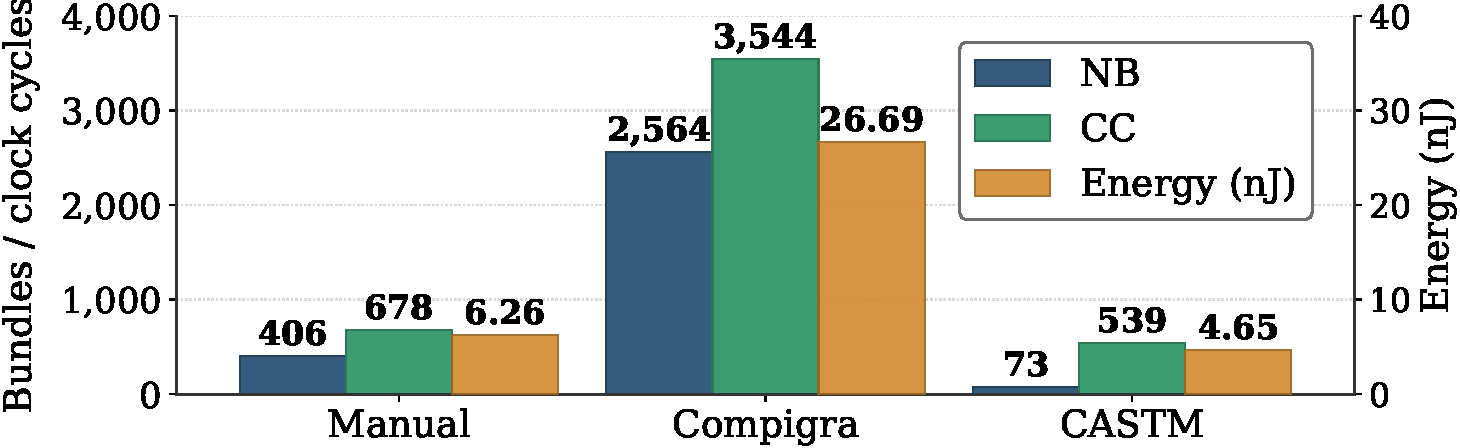
\includegraphics[width=\linewidth]{figures/sbox_compare_plot_v2.pdf}
    \caption{Comparison of the S-box kernel mappings produced by  Manual, Compigra, and \castm{} on the CGRA. Blue and green bars use the left axis and report the number of compiled bundles (NB) and clock cycles (CC), respectively; orange bars use the right axis and report energy (nJoules) per invocation.}
    \label{fig:sbox-comparison}
\end{figure}

Energy per invocation combines the ESL-reported execution energy with the fixed dead-time cost incurred at each CGRA dispatch. This normalization is necessary because the three mappings differ not only in cycle count but also in execution granularity: without accounting for dispatch overhead, a fragmented schedule would understate the system-level cost of repeatedly launching and draining the accelerator.
Idle (\%) in Table~\ref{tab:sbox-comparison} is reported as a bundle-wise geometric mean over per-bundle idle-PE ratios.

\textbf{Compigra cannot map S-box directly.}
The automatic compiler's scheduling heuristic fails on the S-box kernel because Barrett reduction requires cross-PE carry chains and branchless conditional selects that exceed its mapping capabilities.
The workaround is to manually decompose $x^7 \Mod p$ into sub-kernels
and iteratively subdivide when compilation fails---a trial-and-error process that negates the ``automatic'' premise.
The result is \MetricSboxCompigraDispatches{} dispatches with \pct{\MetricSboxCompigraIdlePct} Idle and \pct{\MetricSboxCompigraSmulPct} of SMUL utilization: the hardware multiplier is never used, and the CGRA spends most cycles idle while data is shuffled between dispatches.

\textbf{\castm{} achieves the lowest cycle count.}
The \MetricSboxCastmNB{} compiled bundles (vs.\ \MetricSboxManualNB{} for the Manual schedule) reflect jump-reuse subroutines that share Barrett reduction across the four modular multiplications ($x^2$, $x^3$, $x^4$, $x^7$).
The resulting \cc{\MetricSboxCastmCC} (vs.\ \cc{\MetricSboxManualCC} for Manual) represents a \pct{\MetricSboxCastmCycleReductionPct} cycle reduction attributable to better PE utilization: \pct{\MetricSboxCastmIdlePct} Idle (vs.\ \pct{\MetricSboxManualIdlePct}) and active use of the hardware multiplier (\pct{\MetricSboxCastmSmulPct} SMUL).
Under the energy model, \castm{} also remains the most efficient mapping at \nj{\MetricSboxCastmEnergyNJ}, below Manual at \nj{\MetricSboxManualEnergyNJ} and far below Compigra at \nj{\MetricSboxCompigraEnergyNJ}. The gap is architecturally coherent with the schedules themselves: Compigra expands the kernel into \MetricSboxCompigraDispatches{} dispatches, so its higher energy reflects not only a longer execution (\cc{\MetricSboxCompigraCC}) but also repeated launch and quiescent overheads that are largely avoided by the single-dispatch in the \castm{} schedule.

\textbf{Productivity.}
The Manual approach requires \lines{\MetricLocManual}; \castm{} requires \lines{\MetricLocCastm}---an approximately \timex{\MetricLocCompressionVsManual} reduction.
This gap is structural: \castm{}'s parameterized functions and loop express the kernel once, whereas the hand-written schedule must spell out each PE-cycle placement explicitly, making coding slower and substantially more error-prone.

\textbf{Code complexity.}
Table~\ref{tab:halstead} quantifies complexity using Halstead active volume metric, $V_{\text{act}} = N \log_2 \eta$, where $N$ counts active (non-NOP) tokens~\cite{halstead1977}. We do not report Halstead effort because, for low-vocabulary ISA-level code, it can produce anomalous scaling~\cite{sinha2011}. Owing to explicit per-PE-per-cycle encoding, the Manual schedule reaches \timex{\MetricHalsteadManualRatio} the \texttt{C++} baseline. By absorbing spatial placement and NOP scheduling into the compiler, \castm{} reduces this to \timex{\MetricHalsteadCastmRatio}, corresponding to a \timex{\MetricHalsteadCompressionVsManual} compression factor relative to the Manual schedule. Ideally, Compigra could reduce this complexity to \timex{\MetricHalsteadCompigraRatio} the \texttt{C++} baseline, although at the cost of \timex{\MetricSboxCompigraSlowdownVsCastm} more cycles than \castm{} due to inefficient PE utilization as previously explained.

% AUTO_HALSTEAD_TABLE_BEGIN
\begin{table}[ht]
\caption{Halstead metrics for the S-box kernel. LOC: source lines; $\eta$: unique vocabulary; $N$: active tokens (NOP excl.); $V_{\text{act}}=N\log_2\eta$: active volume~\cite{halstead1977}; Ratio: $V_{\text{act}}$ norm.\ to C++.}
\label{tab:halstead}
\centering
\scriptsize
\setlength{\tabcolsep}{2pt}
\begin{tabular}{@{}l|rrrrr@{}}
\toprule
\textbf{Approach} & \textbf{LOC} & \boldmath{$\eta$} & \boldmath{$N$} & \boldmath{$V_{\text{act}}$} & \textbf{Ratio} \\
\midrule
C++ (Ref.) & 25 & 39 & 104 & 550 & $1.0\times$ \\
Compigra & 47 & 53 & 227 & 1{,}300 & $2.4\times$ \\
Manual CSV & 2{,}030 & 48 & 6{,}348 & 35{,}453 & $64.5\times$ \\
\castm{} (\textbf{Ours}) & \textbf{340} & \textbf{55} & \textbf{607} & \textbf{3{,}509} & $\mathbf{6.4\times}$ \\
\bottomrule
\end{tabular}
\end{table}

% AUTO_HALSTEAD_TABLE_END

\subsection{S-box Configuration Register Pressure}
\label{subsec:creg-analysis}

The S-box kernel also allow us to conduct a controlled sensitivity study for configuration residency. Two implementations bracket the design space: the \emph{Manual} kernel (\MetricSboxManualNB~bundles, flat layout) and the \emph{\castm{}} kernel (\MetricSboxCastmNB~bundles, jump-reuse with shared subroutines). Because the Manual kernel uses only sequential control flow, it can be split into independent sub-kernels at any CRF depth. The \castm{} kernel cannot: its register-indirect returns (\texttt{JUMP~R3}) require all \MetricSboxKernelResidentBundles~bundles to be simultaneously resident in the CRF.

When a kernel of $NB$ bundles exceeds the CRF depth $D$, it must be partitioned into $K = \lceil NB/D \rceil$ sub-kernels. In HEEPsilon's default CMEM organization, each sub-kernel fills an entire memory bank, so every transition between sub-kernels forces the host to reload all configuration data. The overhead decomposes as:
%
{\small
\[
  T_{\mathrm{ovh}} = \underbrace{\textstyle\sum_{i}(s_i\!+\!1)}_{\text{CRF load}} + \underbrace{4(K\!-\!1)}_{\text{controller}} + \underbrace{(K\!-\!1)(16D\!+\!16)}_{\text{CMEM reload}}
\]
}
%
\noindent where the sum runs over the $K{-}1$ transitions ($s_i$ is the size of each reloaded sub-kernel). The first two terms---streaming instructions into the CRF and controller handshake cycles---are small. The CMEM reload term dominates: it transfers the full bank contents via MMIO, costing approximately $16NB$ cycles for a large $K$,
 nearly \emph{constant} regardless of $D$.

At the default $D\!=\!\MetricCrfDefaultDepth$, the Manual kernel loses \pct{\MetricCrfManualDefaultOHPct} of its cycles due to reload overhead ($K\!=\!\MetricCrfManualDefaultK$); doubling or quadrupling $D$ barely helps because the total data volume stays proportional to $NB$. Overhead only vanishes when the entire kernel fits ($K\!=\!1$): this happens for $D\!=\!\MetricCrfDepthFullFit$ in Manual, and $D\!=\!\MetricCrfDepthOneTwentyEight$ in \castm{}. The $5.6\times$ bundle compression from Manual to \castm{} (\MetricSboxManualNB$\to$\MetricSboxCastmNB) now translates into a $4\times$ reduction in CRF requirement, at the cost of \pct{\MetricCrfOneTwentyEightAreaPct} additional area for $D=128$ vs. \pct{\MetricCrfFullFitAreaPct} for $D=512$ (i.e. +\MetricCrfOneTwentyEightExtraFlipFlops~flip-flops vs. +\MetricCrfFullFitExtraFlipFlops~flip-flops on Artix-7 XC7A200T~\cite{xheep}). However, this comes with a rigidity constraint: for any $D < \MetricSboxCastmNB$, the \castm{} kernel cannot execute at all.

\subsection{Poseidon2: RTL Validation}
\label{subsec:rtl-poseidon2}

The S-box CRF-pressure analysis above showed that, for long ZKP kernels, configuration fragmentation and reload overhead dominate before arithmetic throughput can become visible. The full Poseidon2 kernel (366~bundles) requires $D\!=\!\MetricCrfDepthFullFit$ to fit without partitioning.
 Under that condition, we analyze three deployment options when running a batch of Poseidon2 hashes: a \textit{CPU-only} reference that executes all the hashes on the CPU, a \textit{CGRA-only} version that offloads all the hashes to the CGRA, and a \textit{CPU+CGRA} implementation, which evenly launches the hashes concurrently on the CPU and the CGRA. Both \textit{CGRA-only} and \textit{CPU+CGRA} keep the full Poseidon2 kernel on the accelerator.

\begin{table}[!ht]
\caption{Poseidon2: comparison of RTL metrics. T: Time ($\mu$s); Th: Throughput (hashes per sec.); Sp: Speedup; E: Energy ($\mu$J); ES: Energy Savings (\%).}
\label{tab:rtl-performance}
\centering
\footnotesize
\renewcommand{\arraystretch}{1.2}
\setlength{\tabcolsep}{2pt}
\resizebox{\columnwidth}{!}{%
\begin{tabular}{@{}l|ccccc|cccc@{}}
\toprule
\textbf{Config.} & \textbf{T$_{\text{CPU}}$} & \textbf{T$_{\text{CGRA}}$} & \textbf{T$_{\text{tot}}$} & \textbf{Th} & \textbf{Sp} & \textbf{E$_{\text{CPU}}$} & \textbf{E$_{\text{CGRA}}$} & \textbf{E$_{\text{tot}}$} & \textbf{ES} \\
\midrule
\textbf{CPU-only} & \MetricMerkleCpuOnlyProjectedCpuTimePerHashUs & --- & \MetricMerkleCpuOnlyProjectedTimePerHashUs & \MetricMerkleCpuOnlyProjectedHashesPerSec &
1.00 &
\MetricMerkleCpuOnlyCpuEnergyPerHashUJ & --- & \MetricMerkleCpuOnlyTotalEnergyPerHashUJ & 0 \\
\textbf{CGRA-only} & \MetricMerkleOffloadProjectedCpuTimePerHashUs & \MetricMerkleOffloadProjectedCgraTimePerHashUs & \MetricMerkleOffloadProjectedTimePerHashUs & \MetricMerkleOffloadProjectedHashesPerSec & \MetricMerkleOffloadProjectedSpeedup & \MetricMerkleOffloadCpuEnergyPerHashUJ & \MetricMerkleOffloadCgraEnergyPerHashUJ & \textbf{\MetricMerkleOffloadTotalEnergyPerHashUJ} & \textbf{\MetricMerkleOffloadEnergySavingsPct} \\
\textbf{CPU+CGRA} & \MetricMerkleCoexecProjectedCpuTimePerHashUs & \MetricMerkleCoexecProjectedCgraTimePerHashUs & \textbf{\MetricMerkleCoexecProjectedTimePerHashUs} & \textbf{\MetricMerkleCoexecProjectedHashesPerSec} &
\textbf{\MetricMerkleCoexecProjectedSpeedup} &\MetricMerkleCoexecCpuEnergyPerHashUJ & \MetricMerkleCoexecCgraEnergyPerHashUJ & \MetricMerkleCoexecTotalEnergyPerHashUJ & \MetricMerkleCoexecEnergySavingsPct \\
\bottomrule
\end{tabular}
}
\end{table}

The throughput ranking is straightforward. T$_{\text{CPU}}$ and T$_{\text{CGRA}}$ report the time per-hash (full Poseidon2) for which the host CPU and the accelerator are active, with T$_{\text{tot}}$ being the total time per-hash. From this last metric we see that \textit{CPU+CGRA} is the fastest because both devices work in parallel reaching \MetricMerkleCoexecProjectedTimePerHashUs~$\mu$s/hash, the highest throughput, \MetricMerkleCoexecProjectedHashesPerSec~hashes/sec., and up to \MetricMerkleCoexecProjectedSpeedup $\times$ speedup over the \textit{CPU-only}. Interestingly, there is room for improvement for this hybrid deployment because as we see from the T$_{\text{CPU}}$ and T$_{\text{CGRA}}$ times, the workload is currently not balanced between devices. \textit{CGRA-only} also outperforms \textit{CPU-only} at \MetricMerkleOffloadProjectedTimePerHashUs~$\mu$s/hash and  \MetricMerkleOffloadProjectedSpeedup $\times$ speedup.

Energy favors a different organization. E$_{\text{CPU}}$ and E$_{\text{CGRA}}$ represent the energy per-hash consumed by the CPU and CGRA, respectively, while E$_{\text{tot}}$ is the total energy and ES is the energy savings with respect to \textit{CPU-only}. Now, \textit{CGRA-only} reduces the total energy to {\MetricMerkleOffloadTotalEnergyPerHashUJ}~$\mu$J/hash, a \pct{\MetricMerkleOffloadEnergySavingsPct} reduction relative to \textit{CPU-only}, whereas \textit{CPU+CGRA} reaches {\MetricMerkleCoexecTotalEnergyPerHashUJ}~$\mu$J/hash, or \pct{\MetricMerkleCoexecEnergySavingsPct} reduction. In the hybrid deployment, the E$_{\text{CGRA}}$ component is the minimum, but the less efficient E$_{\text{CPU}}$ contribution increases because the CPU computes part of the hashes, which ultimately degrades the total energy.

From  the T$_{\text{CPU}}$ (E$_{\text{CPU}}$) metric in the \textit{CGRA-only} case, we can infer the overhead due to kernel dispatch (input parameters setting + kernel launching + output reading). As we see, this overhead is very low, around 1.3\% (1.5\%) total time (total energy).

In our study, we have found that memory stalls are the most significant source of overhead for this CGRA kernel, representing 23.5\% active cycles. These memory access stalls are mainly due to memory bank conflicts that are even more relevant if other memory subsystem design choices are considered.
For instance, replacing the more flexible host-to-memory crossbar \textit{N:M} that we have considered in this analysis, with the simpler shared path \textit{OneToM}, degrades the \textit{CGRA-only} performance
from \MetricRtlCgraOnlyCC~CC to \MetricRtlCgraOnlyOneToMCC~CC and reduces speedup from \timex{\MetricMerkleOffloadProjectedSpeedup} to \timex{1.06}.

\subsection{Lessons Learned}
\label{subsec:discussion}

Our results provide some interesting architectural lessons. Firstly, CRF configuration capacity is a primary tuning knob: before fragmentation is removed, system behavior is dominated by reload traffic rather than arithmetic execution. Thus, kernels should be designed to fit the CRF as a single unit. Once this requisite is satisfied, throughput and energy do not necessarily favor the same organization of kernels: a hybrid deployment as \textit{CPU+CGRA} provides the highest throughput, whereas \textit{CGRA-only} minimizes total energy consumption. The next optimization step lies less in creating finer-grain offload variants than in reducing the cost of delivering data to an already efficient accelerator by minimizing memory bank conflicts.
Also for hybrid deployments, load-balancing scheduling strategies must be considered.

%!TEX root = main.tex
\section{Conclusions}
\label{sec:conclusion}

In this paper, we have presented \castm{}, the first API targeting the spatial-temporal programming model of CGRA architectures for cryptographic workloads. Specifically, for the BabyBear S-box layer on the  OpenEdgeCGRA architecture, \castm{} achieves a \pct{\MetricSboxCastmCycleReductionPct} cycle reduction over hand-optimized CSV (\cc{\MetricSboxCastmCC} vs. \cc{\MetricSboxManualCC}), while reducing source code by approximately \timex{\MetricLocCompressionVsManual}.

RTL validation of the full Poseidon2 hash function on the ultra-low power HEEPsilon SoC gives us some system lessons. The Configuration Register File capacity is the enabling condition: once the kernel fits in the CRF the running times are no longer masked by reload fragmentation. Under that condition,
offloading the full kernel to the CGRA (\textit{CGRA-only}) minimizes the total energy, whereas a hybrid deployment that computes hashes on the CPU and the accelerator (\textit{CPU+CGRA}) offers the highest throughput.

In summary, we have shown that it is possible to enable privacy-preserving verification on wearable biomedical devices through Zero-Knowledge Proofs, on hardware that is both energy-efficient and with reprogramming capability to track the rapid evolution of ZKP systems.

\textbf{Future work.} Two directions follow: (1)~dual-port SRAM or DMA burst modes to reduce the memory stalls that represent now the main source of overhead;
and (2)~evaluation on alternative ZKP fields (Goldilocks, BN254) and post-quantum workloads to test the generality of \castm{}'s API.


% Acknowledgments section
% Sección de agradecimientos/reconocimientos del trabajo
\section*{Acknowledgments}

Este trabajo ha sido financiado por el XXX (YYYY) a través del proyecto ZZZZ.

\bibliographystyle{Jornadas}
\bibliography{biblio}

\end{document}
